\documentclass[final]{beamer}
\usepackage[size=custom,width=140,height=90,scale=1.15]{beamerposter}

\usetheme{gemini}
\usecolortheme{seagull}
\useinnertheme{rectangles}

\usepackage[utf8]{inputenc}
\usepackage{graphicx}
\usepackage{bm,amsmath,amssymb}
\usepackage{lmodern}
\usepackage[T1,OT1]{fontenc}
\DeclareFontFamily{OMX}{lmex}{}
\DeclareFontShape{OMX}{lmex}{m}{n}{<-> lmex10}{}
\usepackage{hyperref}
\usepackage{booktabs}
\usepackage{tikz}
\usetikzlibrary{shapes.geometric}
\usepackage{listings}
\usepackage{pifont}
\usepackage{caption}
\captionsetup{labelformat=empty, labelsep=none}

\graphicspath{{../paper/images/}}

\hypersetup{
    colorlinks=true,
    linkcolor=blue,
    urlcolor=cyan,
    pdftitle={CALM poster, NeurIPS 2026},
}

\definecolor{codeink}{HTML}{24292F}
\definecolor{codekey}{HTML}{CF222E}
\definecolor{codestr}{HTML}{0A3069}
\definecolor{codecom}{HTML}{6E7781}
\newcommand{\codefont}{\fontencoding{T1}\fontfamily{SourceCodePro-TLF}\selectfont}
\lstdefinestyle{calm}{
  language=Python, basicstyle=\codefont\small\color{codeink}, basewidth=0.6em,
  keywordstyle=\color{codekey}\bfseries, stringstyle=\color{codestr},
  commentstyle=\color{codecom}\itshape, columns=fixed, keepspaces=true, upquote=true,
  showstringspaces=false, numbers=none, aboveskip=0pt, belowskip=0pt}
\lstset{style=calm}

\definecolor{eublue}{HTML}{003399}
\definecolor{euyellow}{HTML}{FFCC00}
\newcommand{\euflag}[1]{%
  \begin{tikzpicture}[x=#1, y=#1, baseline=(current bounding box.center)]
    \fill[eublue] (0,0) rectangle (1.5,1);
    \foreach \k in {0,...,11}
      \node[star, star points=5, star point ratio=2.618, fill=euyellow,
            inner sep=0pt, minimum size=#1/9]
        at ({0.75 + cos(90 - 30*\k)/3}, {0.5 + sin(90 - 30*\k)/3}) {};
  \end{tikzpicture}}

\newcommand{\xb}{\mathbf{x}}
\newcommand{\xbi}{\mathbf{x}_{-i}}
\newcommand{\Xb}{\mathbf{X}}
\newcommand{\gamm}{GA$^2$M}
\newcommand{\gamms}{GA$^2$Ms}
\newcommand{\method}{CALM}
\newcommand{\yes}{\ding{51}}
\newcommand{\no}{\ding{55}}

\newlength{\sepwidth}
\newlength{\colwidth}
\setlength{\sepwidth}{0.025\paperwidth}
\setlength{\colwidth}{0.3\paperwidth}
\newcommand{\separatorcolumn}{\begin{column}{\sepwidth}\end{column}}

\logoright{
\includegraphics[height=6.5cm]{logos/athena-278x300.png}}
\logoleft{%
  \begin{tabular}[c]{c}
    
\includegraphics[width=7cm]{logos/hua-logo.png}\\[1.5ex]
    
\includegraphics[width=5.5cm]{logos/archimedes-logo.png}\\[1.5ex]
    
\includegraphics[height=2.0cm]{logos/lmu_logo.png}
  \end{tabular}%
}
\addtolength{\maxlogowidth}{10ex}

\footercontent{
  Interpretability-by-Design with Conditional Feature Effects \hfill
  NeurIPS 2026, Paris, France \hfill
  \href{mailto:vgkolemis@athenarc.gr}{\texttt{vgkolemis@athenarc.gr}}
}

% ====================
% BibLaTeX
% ====================

\usepackage[backend=biber,
	bibstyle=authoryear,
	citestyle=authoryear,
	style=authoryear,
	maxcitenames=2,
	maxbibnames=20, % limit the length of list of names (authors/editors/etc.)
	sorting=ydnt, % sort references by year (descending), name, title
	dashed=false, % show authors instead of dash in publications having the same authors
	giveninits=true % render authors' given name initials and not the full given names
]{biblatex}
%% Biblatex with Beamer bibliography icons
\setbeamertemplate{bibliography item}{%
	\ifboolexpr{ test {\ifentrytype{book}} or test {\ifentrytype{mvbook}}
		or test {\ifentrytype{collection}} or test {\ifentrytype{mvcollection}}
		or test {\ifentrytype{reference}} or test {\ifentrytype{mvreference}} }
	{\setbeamertemplate{bibliography item}[book]}
	{\ifentrytype{online}
		{\setbeamertemplate{bibliography item}[online]}
		{\setbeamertemplate{bibliography item}[article]}}%
	\usebeamertemplate{bibliography item}}
\defbibenvironment{bibliography}
{\list{}
	{\settowidth{\labelwidth}{\usebeamertemplate{bibliography item}}%
		\setlength{\leftmargin}{\labelwidth}%
		\setlength{\labelsep}{\biblabelsep}%
		\addtolength{\leftmargin}{\labelsep}%
		\setlength{\itemsep}{\bibitemsep}%
		\setlength{\parsep}{\bibparsep}}}
{\endlist}
{\item}
%% Redefine \refname
\renewcommand{\bibname}{References}
%% Redefine \parencite to use square brackets instead of braces
\DeclareCiteCommand{\parencite}
{\usebibmacro{prenote}}
{\usebibmacro{citeindex}%
	\printtext[bibhyperref]{[\usebibmacro{cite}]}}
{\multicitedelim}
{\usebibmacro{postnote}}
%% Highlight author names using Beamer data annotation
%% Usage: add a new line `author+an = {<author-order>=highlight}` to an entry
%% For example: author+an = {3=highlight} => highlight the 3rd author name
\AtBeginBibliography{
	\renewcommand*{\mkbibnamegiven}[1]{%
		\ifitemannotation{highlight}
		{\textbf{#1}}
		{#1}%
	}
	
	\renewcommand*{\mkbibnamefamily}[1]{%
		\ifitemannotation{highlight}
		{\textbf{#1}}
		{#1}%
	}
}

% ====================
% Boxes with tcolorbox
% ====================
\usepackage[most]{tcolorbox}

%%% Beamer colors in boxes

\newcommand{\beamercolorsinboxes}[1]{
	\setbeamercolor{itemize item}{fg=#1!75!black}
	\setbeamercolor{itemize/enumerate body}{fg=#1!65!white}
	\setbeamercolor{itemize/enumerate subbody}{fg=#1!65!white}
	\setbeamercolor{item projected}{fg=white, bg=#1!75!black}
}

%%% Highlight Oval Box
\newtcbox{\xmybox}[1][red]{on line,
	arc=7pt,colback=#1!10!white,colframe=#1!50!black,
	before upper={\rule[-3pt]{0pt}{10pt}},boxrule=1pt,
	boxsep=0pt,left=6pt,right=6pt,top=2pt,bottom=2pt}
%%% Box for stating problems
%%%%%%%%
%Usage: (similar for infobox)
%	\begin{defbox}{title}
	%		contents
	%	\end{defbox}
%%%%%%%%
\newtcolorbox{defbox}[1]{%
	enhanced,
	attach boxed title to top 	left={xshift=5mm,yshift=-5mm,yshifttext=-5mm},
	colback=cyan!5!white,
	colframe=cyan!75!black,
	coltitle=cyan!80!black,
%	left=0mm,right=0mm,top=2mm,bottom=0mm,
	title={#1},
	fonttitle=\bfseries\large, fontupper=\color{cyan!65!white},
	boxed title style={colback=cyan!5!white,colframe=cyan!75!black},
	before upper={
		\beamercolorsinboxes{cyan}
	}
}%
%%% Box for announcement
\newtcolorbox{infobox}[1]{%
	enhanced,
	attach boxed title to top 	left={xshift=5mm,yshift=-5mm,yshifttext=-5mm},
	colback=yellow,
	colframe=red!75!black,
	coltitle=red!75!black,
%	left=0mm,right=0mm,top=2mm,bottom=0mm,
	title={#1},
	fonttitle=\bfseries\large, fontupper=\color{red!65!white},
	boxed title style={colback=yellow,colframe=red!75!black},
	before upper={
		\beamercolorsinboxes{red}
	}
}%
%%% Box for example
\newtcolorbox{exabox}[1]{%
	enhanced,
	attach boxed title to top 	left={xshift=5mm,yshift=-5mm,yshifttext=-5mm},
	colframe=brown!75!black,colback=brown!5!white,coltitle=brown!50!brown!75!black,
%	left=0mm,right=0mm,top=2mm,bottom=0mm,
	title={#1},
	fonttitle=\bfseries\large, fontupper=\color{brown!65!white},
	boxed title style={colback=brown!5!white,coltitle=brown!50!brown!75!black},
	before upper={
		\beamercolorsinboxes{brown}
	}
}%
%%% Theorem Box
%%%%%%%%
%Usage: (similar for conjecture, lemma, etc.)
%	\begin{thm}{title}{nameref}
	%		contents
	%	\end{thm}
% Use \ref{thm:nameref} to refer to the theorem
%%%%%%%%
%%%% Use \newtcbtheorem[number within=section]{thm} to number within each section
\newtcbtheorem[]{thm}%
{Theorem}{attach boxed title to top 	left={xshift=5mm,yshift=-5mm,yshifttext=-5mm},
	enhanced jigsaw,
	%	top=2mm,bottom=0mm,left=0mm,right=0mm,
	fonttitle=\bfseries\large,fontupper=\itshape\color{blue!65!white},
	colframe=blue!75!black,colback=blue!5!white,coltitle=blue!50!blue!75!black,
	boxed title style={colback=blue!5!white,coltitle=blue!50!blue!75!black},
	before upper={
		\beamercolorsinboxes{blue}
	}
}{thm}%
%%% Proposition Box
\newtcbtheorem[use counter from=thm]{prop}%
{Proposition}{attach boxed title to top 	left={xshift=5mm,yshift=-5mm,yshifttext=-5mm},
	enhanced jigsaw,
	%	top=2mm,bottom=0mm,left=0mm,right=0mm,
	fonttitle=\bfseries\large,fontupper=\itshape,
	colframe=gray!75!black,colback=gray!5!white,coltitle=gray!50!gray!75!black,
	boxed title style={colback=gray!5!white,coltitle=gray!50!gray!75!black},
	before upper={
		\beamercolorsinboxes{gray}
	}
}{prop}%
%%% Conjecture Box
\newtcbtheorem[use counter from=thm]{conj}%
{Conjecture}{attach boxed title to top 	left={xshift=5mm,yshift=-5mm,yshifttext=-5mm},
	enhanced jigsaw,
	%	top=2mm,bottom=0mm,left=0mm,right=0mm,
	fonttitle=\bfseries\large,fontupper=\slshape,
	colframe=orange!75!black,colback=orange!5!white,coltitle=orange!50!orange!75!black,
	boxed title style={colback=orange!5!white,coltitle=orange!50!orange!75!black},
	before upper={
		\beamercolorsinboxes{orange}
	}
}{conj}%
%%% Lemma Box
\newtcbtheorem[use counter from=thm]{lem}%
{Lemma}{attach boxed title to top 	left={xshift=5mm,yshift=-5mm,yshifttext=-5mm},
	enhanced jigsaw,
	%	top=2mm,bottom=0mm,left=0mm,right=0mm,
	fonttitle=\bfseries\large,fontupper=\itshape,
	colframe=green!75!black,colback=green!5!white,coltitle=green!50!green!75!black,
	boxed title style={colback=green!5!white,coltitle=green!50!green!75!black},
	before upper={
		\beamercolorsinboxes{green}
	}
}{lem}%
%%% Claim Box
\newtcbtheorem[use counter from=thm]{clm}%
{Claim}{attach boxed title to top 	left={xshift=5mm,yshift=-5mm,yshifttext=-5mm},
	enhanced jigsaw,
	%	top=2mm,bottom=0mm,left=0mm,right=0mm,
	fonttitle=\bfseries\large,fontupper=\itshape,
	colframe=pink!75!black,colback=pink!5!white,coltitle=pink!50!pink!75!black,
	boxed title style={colback=pink!5!white,coltitle=pink!50!pink!75!black},
	before upper={
		\beamercolorsinboxes{pink}
	}
}{clm}%
\renewcommand{\pgfuseimage}[1]{\includegraphics[scale=2.0]{#1}}

\title{Interpretability-by-Design with Accurate Locally Additive Models and Conditional Feature Effects}

\author{Vasilis Gkolemis\inst{1,2} \and
  Loukas Kavouras\inst{2} \and
  Dimitrios Kyriakopoulos\inst{2} \and
  Konstantinos Tsopelas\inst{2} \and
  Dimitrios Rontogiannis\inst{4} \and
  Giuseppe Casalicchio\inst{5} \and
  Theodore Dalamagas\inst{2} \and
  Christos Diou\inst{1,3}
}

\institute[HUA-ATH-MPI-LMU]{
  \inst{1} Department of Informatics and Telematics, Harokopio University of Athens \quad
  \inst{2} IMSI, ATHENA RC \quad
  \inst{3} Archimedes AI, ATHENA RC \quad
  \inst{4} Max Planck ISS \quad
  \inst{5} LMU Munich
}

\date{December 2026}

\begin{document}

\begin{frame}[t,fragile]
  \begin{columns}[t] \separatorcolumn

    \begin{column}{\colwidth}

      \begin{alertblock}{CALM: In a nutshell}
        \Centering
        \Large{\textbf{Interpretable-by-design, without a (high) accuracy tax.}\\[0.4em]
          CALM sits \emph{between} GAMs and \gamms:\\
          close to GAMs in \textbf{interpretability} and close to \gamms{} in \textbf{accuracy}.}
      \end{alertblock}

      \begin{block}{The GAM / GA$^2$M dilemma}
        \begin{itemize}
          \item \textbf{GAMs} ($y = \beta_0 + \sum_i f_i(x_i)$) are fully auditable, one 1D
            curve per feature, but they \textbf{underfit whenever features interact}.
          \item \textbf{\gamms} add pairwise terms $f_{ij}(x_i,x_j)$ and gain accuracy, but
            \textbf{lose two interpretability properties}: (i) a prediction no longer splits
            into one contribution per feature, and (ii) no single plot shows how a feature
            affects the prediction.
          \item \textbf{CALM} keeps univariate shape functions, but allows \emph{several} per
            feature, each active in a different region. Effects stay locally additive, yet
            vary across regions, so interactions are captured without ever leaving 1D plots.
        \end{itemize}

        \begin{figure}
          \centering
          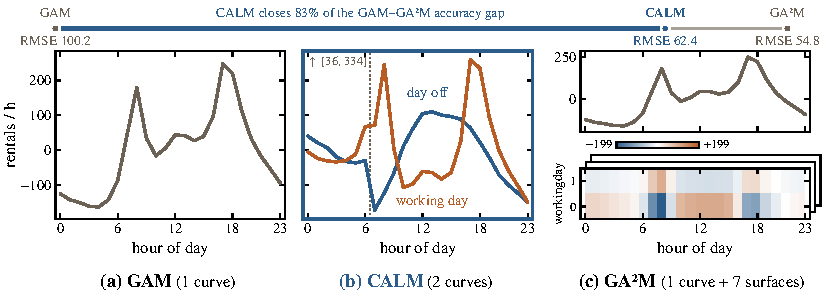
\includegraphics[width=\linewidth]{bike/hero.pdf}
          \caption{The effect of the hour on bike rentals (Bike Sharing). The GAM averages the
            interaction with the working day away, CALM ($d_{\max}=1$) keeps it as two curves,
            and the \gamm{} spreads it over a curve and seven surfaces.}
        \end{figure}
      \end{block}

      \begin{block}{CALM: Model overview}
        On Bike Sharing, the hour splits on the working day: on working days rentals peak at the
        morning and evening commute, whereas on days off they rise to a single broad peak around
        midday.

        \begin{figure}
          \centering
          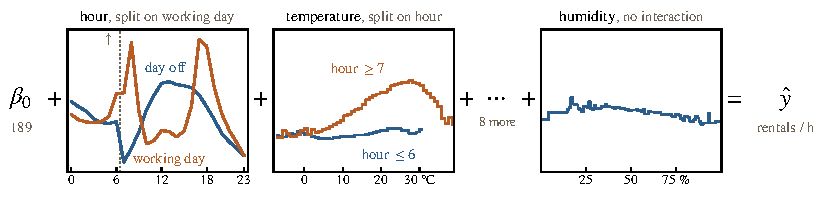
\includegraphics[width=\linewidth]{concept.pdf}
          \caption{The prediction sums one plot per feature, each plot holding one curve per
            region. The temperature splits on the hour; the humidity interacts with no feature
            and keeps one curve.}
        \end{figure}
      \end{block}

      \begin{block}{{\color{teal} How to use CALM}}
        \begin{tcolorbox}[enhanced, width=\dimexpr\linewidth-1.5ex\relax, colback=white,
            colframe=teal!55!black, boxrule=1.2pt, arc=5pt, left=14pt, right=14pt, top=6pt,
            bottom=6pt, middle=4pt, segmentation style={solid, teal!30, line width=1pt}]
          {\codefont\small{\color{codecom}\$} pip install calm-additive}
          \tcblower
\begin{lstlisting}
from calm_additive import CALMRegressor   # or CALMClassifier
calm = CALMRegressor(max_partition_depth=2,  # up to 4 curves per feature
                     teacher="xgb")          # or your own black box
calm.fit(X_train, y_train)
calm.predict(X_test)
calm.print_summary()        # the model on one screen
calm.plot_curves("hour")    # one curve per region
\end{lstlisting}
        \end{tcolorbox}
      \end{block}

    \end{column}
    \separatorcolumn

    \begin{column}{\colwidth}

      \begin{block}{Reading a CALM plot}
        In the CALM panel on the left, each curve is the contribution of the hour in one region: at
        8\,am it is $+246$ on a working day and $-122$ on a day off.

        \smallskip
        Dotted lines mark \emph{hidden jumps}: the temperature and the year split on the hour
        at 6.5, so moving the hour across 6.5 adds a jump in $[36, 334]$ to the change of its
        own curve. Arrows summarize it: $\uparrow$ means $\Delta y > \Delta f_i$, $\downarrow$
        means $\Delta y < \Delta f_i$, $\updownarrow$ means it depends.

        \smallskip
        \begin{center}
        \begin{tabular}{lccc}
          \toprule
          \textbf{Interpretability property} & \textbf{GAM} & \textbf{\gamm} & \textbf{\method} \\
          \midrule
          \textbf{P1} Local feature contribution  & \yes & \no & \yes \\
          \textbf{P2} Regional feature sensitivity & \yes & \no & \yes$^*$ \\
          \textbf{P3} Global feature property (e.g.\ monotonicity) & \yes & \no & \yes \\
          \midrule
          Captures interactions & \no & \yes & \yes \\
          \bottomrule
        \end{tabular}
        \end{center}
        {\small $^*$exact unless the change crosses a dotted line; the arrows still answer
        qualitative questions. In a \gamm{} the contribution is not even unique.}
      \end{block}

      \begin{block}{Humans actually read CALM plots better}
        In a within-subjects user study ($N=25$), participants answered questions on the effect
        of the hour in a Bike Sharing model, once from CALM's curves and once from a \gamm's
        curve and heatmaps. They answered \textbf{54\,\%} correctly with CALM and \textbf{34\,\%}
        with the \gamm{} ($p<0.05$), and the gap is widest on how long the hour takes to lower
        the prediction (\textbf{40\,\%} vs.\ \textbf{12\,\%}). The advantage holds among the 13
        advanced or expert participants (65.4\,\% vs.\ 30.8\,\%).
      \end{block}

      \begin{defbox}{CALM: Conditionally Additive Local Models}
        \begin{equation*}
          g\left(\mathbb{E}[Y \mid \Xb = \xb]\right)
            \;=\; \beta_0 + \sum_{i=1}^{d} f_i^{\,(r_i(\xbi))}(x_i)
        \end{equation*}
        \begin{itemize}
          \item \textcolor{blue}{\textbf{Conditional feature effects.}} Each feature $i$ owns a
            \emph{set} of univariate shape functions $\{f_i^{(r)}\}_{r=1}^{R_i}$.
          \item \textcolor{blue}{\textbf{Region selection.}} $r_i(\xbi)$ picks which curve is
            active, based only on the other features.
          \item \textcolor{blue}{\textbf{Readable regions.}} Each region is a conjunction of at
            most $d_{\max}$ threshold rules, read off a tree $T_i$ over $\xbi$:
            $\;\mathcal{R}_i^{(r)} = \{\, \xbi \mid \wedge_k (x_{j_k}\,\text{op}_k\,\tau_k) \,\}$.
            So CALM captures interactions of up to $d_{\max}+1$ features.
          \item \textcolor{red}{\textbf{Cheap expressivity.}} Each feature has at most
            $2^{d_{\max}}$ curves, yet every instance picks one region per feature, so the curves
            combine into up to $2^{d\cdot d_{\max}}$ distinct additive models.
          \item \textcolor{blue}{\textbf{Two knobs.}} They bound what a reader must inspect:
            $d_{\max}$ (2 by default) caps how many curves each feature has and $K$ how many
            interactions the model captures in total.
        \end{itemize}
      \end{defbox}

      \begin{block}{Training: a 3-step distillation pipeline}
        \textbf{\textcolor{blue}{Step 1: Reference model.}} \\
        Fit a black box $f_{\texttt{ref}}$ (XGBoost by default).
        It is used \emph{only} to detect interactions, then discarded.

        \vspace{1.0em}
        \textbf{\textcolor{red}{Step 2: Find near-additive regions.}} \\
        Interactions show up as \emph{heterogeneity} of the local effects $h$ of $x_i$ around
        their average $\mu_i^{\mathcal{R}}$:
        \begin{equation*}
          H_i^{\mathcal{R}} \;=\; \sqrt{\mathbb{E}\!\left[\big(h(X_i,\Xb_{-i}) - \mu_i^{\mathcal{R}}(X_i)\big)^2\right]},
          \qquad \Xb_{-i}\in\mathcal{R}.
        \end{equation*}
        A CART-style tree $T_i$ per feature splits on the $x_j$ that most reduces
        $H_i^{\mathcal{R}}$. Then a greedy selection keeps only the trees that improve an
        additive surrogate of $f_{\texttt{ref}}$, so a redundant tree is discarded and CALM stays
        small. Under specific assumptions, CALM's error in approximating $f_{\texttt{ref}}$ is at
        most $d$ times the sum of the squared heterogeneities, so partitioning tightens this bound.

        \vspace{1.0em}
        \textbf{\textcolor{magenta}{Step 3: Region-aware backfitting.}} \\
        Shape functions are fitted by gradient boosting, each update restricted to its own
        region. Regions differ across features, so the updates are \emph{coupled}: a single
        additive predictor with region-gated components, whose idealized version converges to
        an empirical risk minimizer over the fixed-tree CALM class.
      \end{block}

      \vspace{0.5ex}
      \begin{columns}[c]
        \begin{column}{0.12\linewidth}
          \euflag{2.6cm}
        \end{column}
        \begin{column}{0.86\linewidth}
          {\scriptsize Funded by the European Union under Grant Agreements No.~101289094 (AIRIS)
          and No.~101135826 (AIDAPT). Views and opinions expressed are however those of the
          authors and do not necessarily reflect those of the European Union or the granting
          authority (HaDEA). Neither the European Union nor the granting authority can be held
          responsible for them.\par}
        \end{column}
      \end{columns}

    \end{column}
    \separatorcolumn

    \begin{column}{\colwidth}

      \begin{block}{CALM: Paper \& Code}
        \begin{itemize}
          \item \textbf{Paper:} \quad \href{https://arxiv.org/abs/2602.16503}{\texttt{arxiv.org/abs/2602.16503}}
          \item \textbf{Page and docs:} \quad \href{https://givasile.github.io/calm-additive}{\texttt{givasile.github.io/calm-additive}}
          \item \textbf{Package:} \quad \href{https://github.com/givasile/calm-additive}{\texttt{github.com/givasile/calm-additive}}
          \item \textbf{Experiments:} \quad \href{https://github.com/givasile/calm-paper}{\texttt{github.com/givasile/calm-paper}}
        \end{itemize}
      \end{block}

      \begin{block}{Synthetic tasks: near-GA$^2$M accuracy, simpler explanation}
        Three independent features $x_i \sim \mathcal{U}(-1,1)$, one interaction per case: in
        Case 1, $x_3$ switches shape on the sign of $x_2$; in Case 2, on the signs of $x_1$ and
        $x_2$, which a \gamm{} cannot express; in Case 3, $x_2$ and $x_3$ interact as a smooth
        product, which CALM approximates by regions.

        \begin{figure}
          \centering
          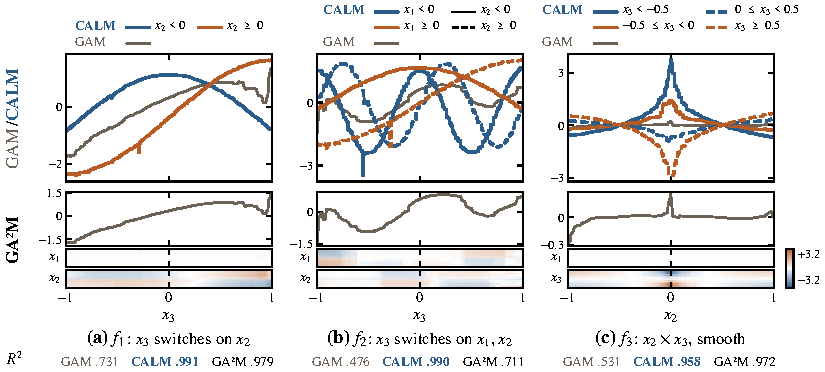
\includegraphics[width=\linewidth]{custom-visuals/synthetic.pdf}
          \caption{Top: CALM's curves, one per region, over the GAM's single curve (gray).
            Bottom: the \gamm's main curve and its two heatmaps, three views to combine per
            feature.}
        \end{figure}
        The GAM misses every interaction. CALM matches the \gamm{} in Case 1, is far more
        accurate in Case 2 and slightly below it in Case 3.
      \end{block}

      \begin{block}{Real datasets: 24 tabular tasks}
        We compare CALM with the black box XGBoost, two GAMs and two \gamms{} over 5-fold CV,
        with no tuning per dataset. A win or a loss counts only when two means differ by more than
        the larger of their standard deviations.

        \smallskip
        \begin{center}
        \setlength{\tabcolsep}{12pt}
        \begin{tabular}{lccccc}
          \toprule
          \textbf{CALM wins/draws/losses} & \textbf{BB} & \multicolumn{2}{c}{\textbf{GAM}} & \multicolumn{2}{c}{\textbf{GA$^2$M}} \\
          \cmidrule(lr){2-2} \cmidrule(lr){3-4} \cmidrule(lr){5-6}
          & \textbf{XGB} & \textbf{NAM} & \textbf{EBM} & \textbf{EB$^2$M} & \textbf{NODE} \\
          \midrule
          Classification (10) & 1/5/4  & 5/5/0  & 3/7/0 & 0/7/3 & 1/7/2 \\
          Regression (14)     & 2/1/11 & 10/4/0 & 8/6/0 & 1/5/8 & 4/6/4 \\
          \bottomrule
        \end{tabular}
        \end{center}

        \begin{itemize}
          \item \textbf{Never behind a GAM:} CALM closes a median 37\,\% of the GAM to XGBoost
            gap in regression and 31\,\% in classification.
          \item \textbf{Competitive with \gamms:} it matches or beats NODE-GA$^2$M on most
            datasets; EB$^2$M is more accurate on 8 of the 14 regression datasets, the cost of
            1D curves instead of 2D surfaces.
          \item \textbf{Sparser \& faster:} CALM adds 8.2 curves to the GAM in regression and 7.9
            in classification, against 14.3 and 15.2 EB$^2$M surfaces; it fits 19 of the 24
            datasets in under a minute (median 21\,s).
          \item \textbf{Stable:} on 77\,\% of the 376 features, all 5 fold refits agree on whether
            to split the feature (90\,\% on at least 4).
        \end{itemize}
      \end{block}

      \begin{alertblock}{Takeaway}
        \Centering
        \large{A new model class between GAMs and \gamms:\\
        \textbf{it never loses to a GAM, and it is read more accurately than a \gamm.}}
      \end{alertblock}

    \end{column}
    \separatorcolumn
  \end{columns}

\end{frame}

\end{document}
